\section{Game Architecture}
Our architecture is built as follows: we have a controller type, the game state, the rendering logic and a simulator. 

\begin{figure}[htbp]
	\centering
	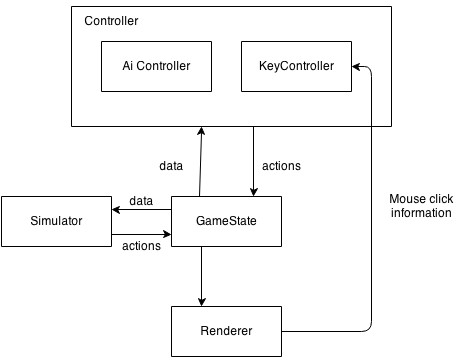
\includegraphics[scale=1]{CZHV_Diagram.png}
	\caption{current program design.}
\end{figure}

\FloatBarrier

\section{Controller}
This is an object that can be extended to various types of controllers. We used an AI controller and an input controller, however it could also be extended to a networked controller for multiplayer. The AI controller consists of an AI manager and an AI implementation. These will be treated in greater detail in the AI section.
\section{Simulator}
Our simulator is different from the intended simulator. This simulator runs autonomous routines on a different thread modifying the game-state using the defined routines. One major part of our simulator is the flocking routine. This calculates and applies the flocking vectors. We also hoped that we could apply our actions in this part, however this would cause concurrency problems with the renderer, thus we made the game-state self-updating with the given actions. More on the actions in the following section. We also had some concurrency problems with the flocking routine, however the chance this occured was extremely low with very specific conditions which we still do not understand and as such we have left it in the simulator thread. Flocking and the pathfinding algorithms are discussed in more detail later.
\section{GameState}
This part defines the state of the game for instance it contains the map data, the locations of the characters and a queue with actions in need of processing. The renderer will read this state and update the view and the controllers and the simulator will produce actions and push them onto the queue in order to update the game state. The actions are implemented similarly to the Mediator pattern. The actions themselves are "mediators" between the game state and the controllers or the simulator.
This ensures that there are no concurrency issues and there have been no other issues using this design. Moreover this also means that our program becomes very extensible, we can add more simulators or controllers fairly easily. The simulator and controllers one can push a new action onto the queue when necessary and can continue with their other tasks as the action is guaranteed to perform. For the MoveTo and GroupMove actions some form of feedback might be necessary in order to check whether a viking or zombie is near or at their destination if this information is relevant. However this information is also readily available in the game state and can be polled if required. 
\section{Renderer}
This provides our rendering logic. It combines the data from the game state with drawing routines and applies various rendering techniques. These rendering techniques will be discussed in detail in the computer graphics section.
